
\chapter{Motivation}
\label{chap:motivation}


As described in chapter~\ref{chap:virt}, hypervisors virtualize local storage resources by mapping guest storage devices onto files in their local filesystem, in a method commonly referred to as a nested filesystem~\cite{le12nested}. As a result, they replicate the guest operating system's (OS) software layers that abstract and secure the storage devices. Notably, these software layers have been shown to present a performance bottleneck even when not replicated~\cite{yu14swoverheads}, due to the rapid increase in storage device bandwidth ~\cite{intel-ssd,seagate16ssd}.
%
Moreover, further performance degradation is caused by the method by which hypervisors virtualize storage devices and the resulting communication overheads between the guest OS and the underlying hypervisor.
Consequently, the storage system is becoming a major bottleneck in modern virtualized environments.
%
In this section we examine the sources of these overheads and outline how they can be mediated using a self-virtualizing storage device.

% software layers
Prevalent storage devices present the software stack with a raw array of logical block addresses (LBA), and it is up to the OS to provide a flexible method to partition the storage resources into logical objects, or files. In addition, the OS must enforce security policies to prevent applications from operating on data they are not allowed to operate on.
%
The main software layer that provides these functionalities is the filesystem, which combines both allocation and mapping strategies to construct logical objects and map them to physical blocks (for brevity, we focus the discussion on these two functionalities and ignore the plethora of other goals set by different filesystems). In addition, the filesystem layer also maintains protection and access permissions. Besides the filesystem, another common layer is the block layer, which caches disk blocks and abstracts the subtleties of different storage devices from the filesystem layer.

When an application accesses a file, the OS uses the filesystem layer to check the access permissions and map the file offset to an LBA on the storage device. It then accesses its block layer, which retrieves the block either from its caches or from the physical device. In a VM, this process is replicated since the storage device viewed by the guest OS is actually a virtual device that is mapped by the hypervisor to a file on the host's storage system. Consequently, the hypervisor invokes its own filesystem and block layers to retrieve the data to the guest OS. 

% virtualization method

%%%%%%%%%%%%%%%%%%%%%%%%%%%%%%
\begin{figure}[t]
  \centering
  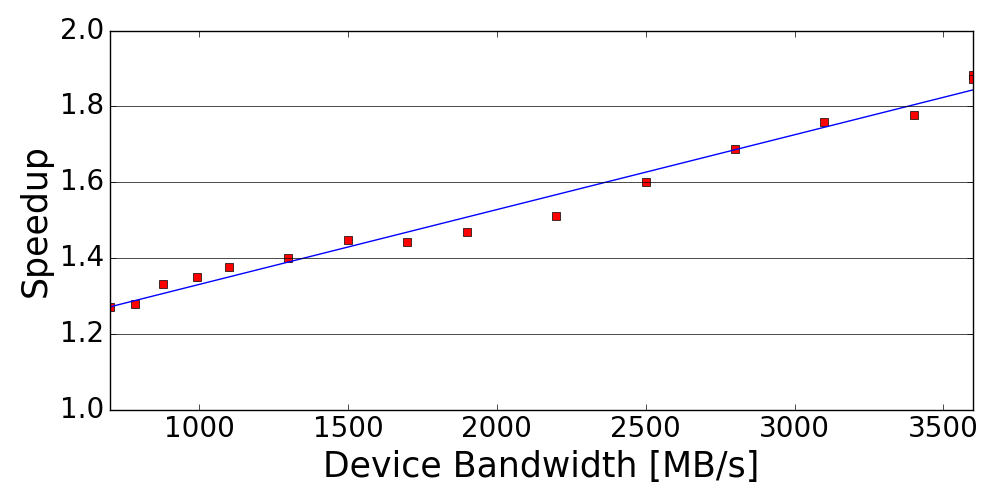
\includegraphics[width=\columnwidth]{figs/motivation.png}
  \caption{The performance benefit of direct device assignment over virtio for high-speed storage devices. Fast devices were emulated using an in-memory disk (ramdisk) whose bandwidth peaks at 3.6GB/s.
    \label{fig:directperf}}
  \end{figure}
%%%%%%%%%%%%%%%%%%%%%%%%%%%%%%

% quantify the overheads
Figure~\ref{fig:directperf} quantifies the potential bandwidth speedup of direct device assignment over the common virtio interface for high-speed storage devices. We have emulated such devices by throttling the bandwidth of an in-memory storage device (ramdisk). Notably, due to OS overhead incurred by its software layers, the ramdisk bandwidth peaks at 3.6GB/s. 

The figure shows the raw write speedups obtained using direct device assignment over virtio for different device speeds, as observed by a guest VM application.
Notably, we see that compared to the state-of-the-art virtio method, direct device assignment roughly doubles the storage bandwidth provided to virtual machines for modern, multi GB/s storage devices.
The reason for these speedups is that as device bandwidth increases, the software overheads associated with virtualizing a storage device become a performance bottleneck.
Using the direct device assignment method eliminates both the virtualization overheads as well as the overheads incurred by the replication of the software layers in the hypervisor and the guest OS.

% we need NeSC
The potential performance benefits of direct device assignment motivate the incorporation of protection and isolation facilities into the storage device. These facilities will enable multiple guest VMs to share a directly accessed physical device without compromising data protection.

%%%%%%%%%%%%%%%%%%%%%%%%%%%%%%
\begin{figure}[t]
  \centering
  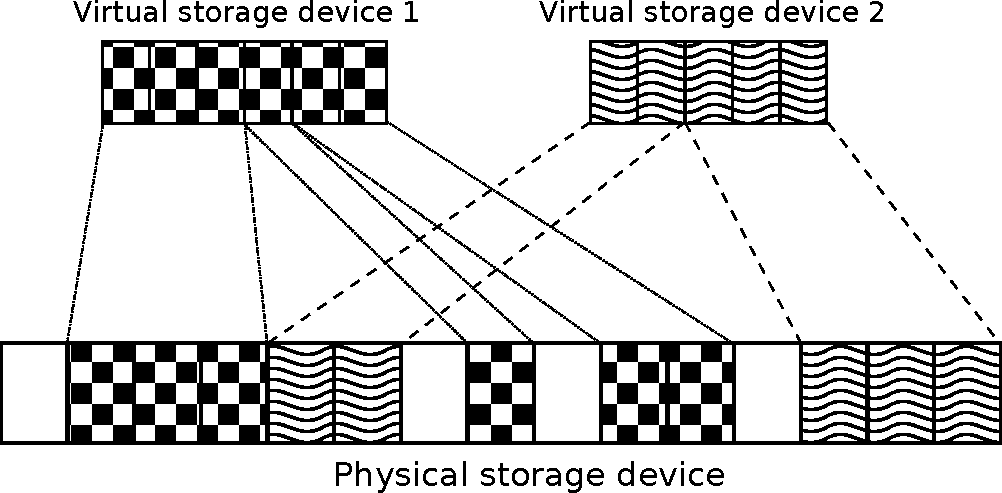
\includegraphics[width=\columnwidth]{figs/nesc-overview.pdf}
  \caption{Exporting files as virtual devices using NeSC.\label{fig:nesc_outline}}  
\end{figure}
%%%%%%%%%%%%%%%%%%%%%%%%%%%%%%

This research presents the nested storage controller (NeSC), which enables multiple VMs to concurrently access files on the host's filesystem without compromising storage security (when NeSC manages a single disk, it can be viewed simply as a PCIe SSD).
Figure~\ref{fig:nesc_outline} illustrates how NeSC provides VMs with secure access to a shared physical device.
NeSC leverages the SR-IOV features of the PCIe gen3~\cite{pcisigiov} to export host files as multiple virtual devices on the PCIe address space. Each virtual device is associated with a collection of non-contiguous blocks on the physical device, which represent a file, and is prevented from accessing other blocks. VMs can therefore directly access the virtual device and bypass the virtualization protocol and hypervisor software (notably, NeSC is compatible with the modern NVMe standard~\cite{nvme}).

%%The rest of this paper describes the design, architecture, and evaluation of NeSC.



